\documentclass[12pt]{article}
\usepackage{geometry}                % See geometry.pdf to learn the layout options. There are lots.
\geometry{a4paper}                   % ... or a4paper or a5paper or ... 
\usepackage{graphicx}
\usepackage{amssymb}
\usepackage{amsthm}
\usepackage{epstopdf}
\usepackage[utf8]{inputenc}
\usepackage[gen]{eurosym}
\usepackage[usenames,dvipsnames]{color}
\usepackage[table]{xcolor}
\usepackage{hyperref}
\DeclareGraphicsRule{.tif}{png}{.png}{`convert #1 `dirname #1`/`basename #1 .tif`.png}

\theoremstyle{definition}
\newtheorem{example}{Example}

\newenvironment{explanation}{%
   \setlength{\parindent}{0pt}
   \itshape
   \color{blue}
}{}

\newcommand{\projectname}{Nao Soccer}
\newcommand{\productname}{Nao Soccer}
\newcommand{\projectleader}{Viktoria Streibl, Melanie Mühleder, Sabina Brantner}
\newcommand{\documentstatus}{In progress}
%\newcommand{\documentstatus}{Submitted}
%\newcommand{\documentstatus}{Released}
\newcommand{\version}{V. 1.0}
\newcommand{\unclear}[1]{\vspace{.5em}\parbox{.9\linewidth}{\color{red}{\bf Remark: #1}}\vspace{.5em}}

\begin{document}
\begin{titlepage}
\begin{flushright}

\includegraphics[scale=.5]{htlleondinglogo.png}\\
\end{flushright}

\vspace{10em}

\begin{center}
{\Huge Project Proposal} \\[3em]
{\LARGE \productname} \\[3em]
\end{center}

\begin{flushleft}
\begin{tabular}{|l|l|}
\hline
Project Name & \projectname \\ \hline
Project Leader & \projectleader \\ \hline
Document state & \documentstatus \\ \hline
Version & \version \\ \hline
\end{tabular}
\end{flushleft}

\end{titlepage}
\section*{Revisions}
\begin{tabular}{|p{.25\linewidth}|p{.3\linewidth}|p{.37\linewidth}|}
\hline
\cellcolor[gray]{0.5}\textcolor{white}{Date} & \cellcolor[gray]{0.45}\textcolor{white}{Author} & \cellcolor[gray]{0.5}\textcolor{white}{Change} \\ \hline
September 3, 2016&V. Streibl, M. Mühleder, S. Brantner&Extended and cleared System Concepts \\ \hline
September 1, 2016&V. Streibl, M. Mühleder, S. Brantner&Extended and cleared System Concepts \\ \hline
August 31, 2016&V. Streibl, M. Mühleder, S. Brantner, P. Bauer&More content in objectives and system concepts and consolidation \\ \hline
August 18, 2016&P. Bauer&Wording \\ \hline
August 17, 2016&V. Streibl, M. Mühleder, S. Brantner, P. Bauer&First version \\ \hline
\end{tabular}
\pagebreak

\setcounter{tocdepth}{2}
\tableofcontents
\pagebreak

\section{Management Summary}\label{sec:managementsummary}
This proposal describes a project which should push forward the development of robotic software at the HTL Leonding. In particular we want to achieve two goals:

\begin{itemize}
	\item {\em Participation in the RoboCup 2017 and/or 2018.} The RoboCup is a worldwide robot competition with a number of several different disciplines. We want to participate in the so-called {\em Standard Platform League (SPL)}, which is a robot soccer league where all teams have to use a standard hardware~\cite{softbank_robotics_who_2016} and only compete in terms of different software. The software has to control the robots autonomously, i.e., that no possibilities for remote control or other external help are allowed. We plan to establish a software by December 1, 2016 to apply for the participation at the SPL 2017 . In case of a successful application it is planned to take part in the SPL 2017 at Nagoya, Japan, as the first and only school worldwide which does not have a university level.
	
	\item {\em A significant stabilization of the demonstration software.} The Naos are a central point of the appearance of the HTL Leonding at official events. The software used so far for such events was unstable, hard to use and required a steep learning curve for students to do these demonstrations. The demonstration platform developed by the authors of this proposal during the last year shall be further stabilized and refined.
\end{itemize}

The soccer part of the project needs a set of supporting measures which can be split into two phases. Phase 1 starts immediately and has the goal to apply for the SPL 2017. The second phase will start on December 20, 2017 and has the goal to establish an effective Nao team for the SPL 2017. It has to be mentioned that Phase~2 will only start in its full form if we succeed to apply for then SPL.

\begin{itemize}
	\item Phase 1
    	\begin{itemize}
            	\item Two Nao Robots as replacements for the existing ones
		\item Auxiliary batteries for the robots
            	\item A playing field in size and form of the fields used at the competitions
		\item A space to work
            	\item Web site
    	\end{itemize}
	\item Phase 2
	\begin{itemize}
            	\item Four more Robots for the competition. A total number of six fully working robots is necessary.
            	\item Auxiliary batteries for the new robots
            	\item Coverage of travel costs
		\item Jerseys for the Naos and the humans
	\end{itemize}
\end{itemize}

\section{Initial Situation}
The HTL Leonding is already involved in the topic of robotics since several years. One of the highlights of the efforts done in this field so far was the participation in RoboCup competitions. Especially during the years 2008 to 2010 some awards were won in the MiroSot league~\cite{fira_micro_2014}. Furthermore, robots are a central part in all official promotion events of the HTL Leonding and serve as an effective eye catcher.

In the meanwhile the RoboCup competitions changed significantly and a good part of them nowadays focus on soccer for humanoid robots. Therefore our school purchased three Nao robots~\cite{softbank_robotics_who_2016} during the years 2009 and 2010 to evaluate the possibility to participate in the new competitions called the {\em Nao Standard Platform League (SPL)}. In this league all participating teams have to use the same hardware (the Nao robots produced by SoftBank Robotics) and the teams differ only in the quality of their software. More details about the SPL can be found at~\cite{spl_standard_2016}.

From this time onwards several student projects were done to get more expertise in this field but until now it was impossible to get a software done which would be competitive in the RoboCup challenges. Last year the authors of this proposal have taken over this field, have collected the available software and since then push forward a working code base for the Naos. During the last year we were able to implement a system to support demonstration of Nao capabilities at marketing events. In particular a server holding Nao apps and an Android app by which these apps can be downloaded easily to the Nao was developed. This software will be used during the next official events of our school.

During the last year the plan evolved to take part in the SPL, therefore, we visited the RoboCup 2016 in Leipzig. During this visit we gained a lot of impressions and we were able to talk to several teams which shed some clearer light how we can accomplish a successful application for the RoboCup 2017.

As previously mentioned the available Naos were purchased in the years 2009 and 2010 and gained already a significant age. Particularly all the Naos ran out of maintenance support by SoftBank Robotics. Currently we are still able to work with the newer two of our robots. The oldest can hardly be used anymore since it uses an AMD GEODE CPU which is not supported by NAOqi 2.x anymore~\cite{inbar_new_2014}. But it can be foreseen that also the newer robots will not be usable for a longer time anymore since from our experience it is necessary to send them for maintenance every two years in order to keep them in a workable state.

 
\section{General Conditions and Constraints}
\subsection{Organizational}
% Welcher Rahmen steht uns zur Verfügung? Nur Syp oder auch Dipl?
\subsubsection{Due Dates}
The following table gives an overview of the most important due dates for the next year:

\begin{tabular}{|p{.21\linewidth}|p{.3\linewidth}|p{.38\linewidth}|}
\cellcolor[gray]{0.5}\textcolor{white}{Date} & \cellcolor[gray]{0.43}\textcolor{white}{Event} & \cellcolor[gray]{0.5}\textcolor{white}{Remarks} \\ \hline
October 12 to October 15, 2016 & Messe ``Jugend und Beruf'' 2016 & Fair where our school takes part in and where the Naos are used to attract new students. \\ \hline
November 1, 2016 & Official release of call for application and rule set 2017 & Typically the rule set is more a pre-release and given as a delta to the rule set of 2016. \\ \hline
December 1, 2016 & Due date for applications & The application for the RoboCup 2017 has to be submitted.\\ \hline
December 20, 2016 & Qualification announcement deadline & The teams who successfully qualified are announced.\\ \hline
January 26 and 27, 2017 & ``Tag der offenen Tür'' & Open house at our school to present the best to interested new students.\\ \hline
July 27 to 30, 2017 & RoboCup 2017, Nagoya, Japan & The next years competition\\ \hline
\end{tabular}
\\

It has to be noticed that the time frame between the official announcement of the new rule set and the due date for application is pretty narrow. Therefore, we tried to get some preview which result will be presented in section~\ref{sec:technical}.

According to the {\em Call for Application for Participation} of last year~\cite{robocup_2016_standard_platform_league_call_2015} the core part of the application has to be a video which demonstrates the ability of the team to play soccer. The footage of a length of max. five minutes has to show at least one robot attempting to kick off and score. Furthermore it is very likely that the technical committee of the RoboCup wants to get a live demonstration of the soccer capabilities via a live telephone conference which is expected to take place in the first half of December 2016.

\subsubsection{Available Person Power}
The current team consists of three students and a supervising teacher. This means that a total time budget of not more than 20 hours per week as an average can be estimated.

\subsection{Technical}\label{sec:technical}
The detailed list of all technical constraints known so far is listed in the current Nao SPL rule book~\cite{robocup_technical_committee_robocup_2016}. For the 2017 competition some changes are announced. We will list these changes here and furthermore some of the constraints as far as they need special concern.

\subsubsection{Necessary Naos}
A team taking part in the SPL has to consist of five Naos, one goal keeper and four field players. All these robots have to be of grey color. Additionally a sixth Nao could be used as a coach. It is estimated that, for a fully functional team, a set of at least six Naos is necessary. The whole team has to wear jerseys which are same colored and numbered from 2 to 5 and the goal keeper has the number 1. A number 6 may be used for a substitute player that enters the game later.

\subsubsection{Indoor Competition Only}
Since 2016 an outdoor competition is held where the Naos have to deal with outdoor light conditions. We plan to participate only in the indoor competition although the indoor competition will be brought closer to natural light conditions (see also section~\ref{sec:light}).

\subsubsection{Field Surface}
According to the pre-announcement of the 2017 rules the game will switch the field surface to 8mm artificial turf (similar to what was used in the 2016 SPL outdoor competition).

\subsubsection{Light Conditions}\label{sec:light}
Furthermore it is announced that the playing fields will be move towards more natural lighting (full details in Nov 1 rulebook draft). Natural lighting will become more of a factor (as we will likely either be next to windows or in an arena with natural lighting).

\section{Project Objectives and System Concepts}
The objectives of this project can be split into three main points:
\begin{itemize}
	% \item Schönes Sarkasmus-Schild
	\item Qualification for the SPL
	\item Support the school at official events 
	\item Participation in the competition 2017 and/or 2018
\end{itemize}


\subsection{Qualification for the SPL}
By December 1 we have to get a software ready which, at least, controls the Nao such that it can kickoff a ball and then score a goal. The whole scenario has to take place on a standard, i.e., 9 m x 6 m field as used for the competition. The following goals have to be achieved to accomplish this.
\begin{itemize}
	\item Analyses of Software used in 2016
	\item Vision: Recognition of ball, goal(s), and lines; analysis of the capabilities of the robot cameras
	\item Kicking the ball
\end{itemize}

\subsubsection{Analyses of Software Used in 2016}
Since all teams taking part in the RoboCup competition are requested to publish their software we will take this and start out by analyzing the software of the best teams of the competition 2016. Here we list the teams which software we want to investigate in particular and also the reasons why we chose these teams. Although the informal preview of the rule set for 2017 states that the amount of code used from other teams may be limited, we will take as much as possible and then adapt to the actual regulations as soon as they are released.

\begin{itemize}
	\item {\em B-Human} This team won the competition 2016.
	\item {\em U-Chile} Had a strong team and convinced during the second day of the competition 2016. Unfortunately the performance dropped significantly in the finals. We suspect a bad adaption of the vision configuration.
	\item {\em UNSW-Australia} In this team we observed one of the most stable walks.
	\item {\em UT-Austin} We observed a  good field scan (and therefore a pretty sophisticated self location and orientation of the Naos) and the indoor walk is more stable than the walk of UNSW-Australia
\end{itemize}

\subsubsection{Basic Walk and Kick}
Analysis of the competition 2016 has shown that several teams had troubles to keep the Naos in balance when they were kicking. So it is the main goal here to keep the Naos stable when they kick. It is planned to start off by analyzing the walks of the last year's successful teams and to adapt these to the new surface conditions. For a first attempt we do not concentrate on high energy efficiency since this will get of higher importance during a full length match.

\subsubsection{Vision}
A crucial part of the whole player software is the vision system. The hard part is to distinguish between the field lines, the goal, the ball, and the Naos which are all (more or less) white colored. The standard image detection/recognition library used on the Naos is OpenCv. It will be necessary to get in a good command of this library and the techniques it provides.

Furthermore it is assumed to be helpful to get a good understanding of the constraints of the camera hardware on the Naos. We want to understand within which distances the Naos are able to recognize a ball, a goal, another robot, etc.

\subsection{Support the School at Official Events}
Besides the goals directly related to the participation in the RoboCup 2017 we will support our school by taking part in two official events of the HTL Leonding.
\subsubsection{Messe ``Jugend und Beruf 2016'' Wels}
This fair will take place from October 12 to 15, 2016. Since we cannot expect to have significant software parts for playing soccer by October and, furthermore, due to space limitations at our booth we will present the project we developed during last school year. This includes the app {\em NaoRemote} to control the Naos via an Android device. Additionally we want to show some dances.

\subsubsection{``Tag der offenen Tür'' at the HTL Leonding}
At this event we already expect to have some soccer software ready to be demonstrated. At least we want to show the visitors the software to be ready for the application to the competition 2017. 

\subsection{Participation in the Competitions 2017 and/or 2018}
If we win the participation in one of the competitions of the next years we need to have a fully working team of five Naos. In order to come into this position we expect the following goals to be achieved. The goals are listed in a timely order as we expect that we need to tackle them.

\subsubsection{Advanced Walk and Kicks}
Based on the work done to get qualified for the RoboCup 2017 we will have to do optimizations concerning energy efficiency and temperature. During last years competition it became obvious that a mean energy efficiency which resulted in high joint temperatures caused a significant loss in stiffness of the joints which itself caused high instabilities of the robots. Furthermore, it was observed that some teams gained competitive advantage by having the possibility to do alternative kicks. Therefore it is planned to implement kicks to the side or kicks to the back.

\subsubsection{Show Robot Status}
To quickly monitor the status of the Naos, we plan to implement some status indicators via coloring its eyes. The following table represents some first ideas which status could be interesting to facilitate our development and how we want to indicate with two eyes colors.
\\[1em]
\unclear{In the next table: What is if the Nao sees the goal? What means the red/red status? What do you mean by ``the x/y state is necessary?}
\\
\unclear{Please check if the state diagram is okay, and the table beneath}\\
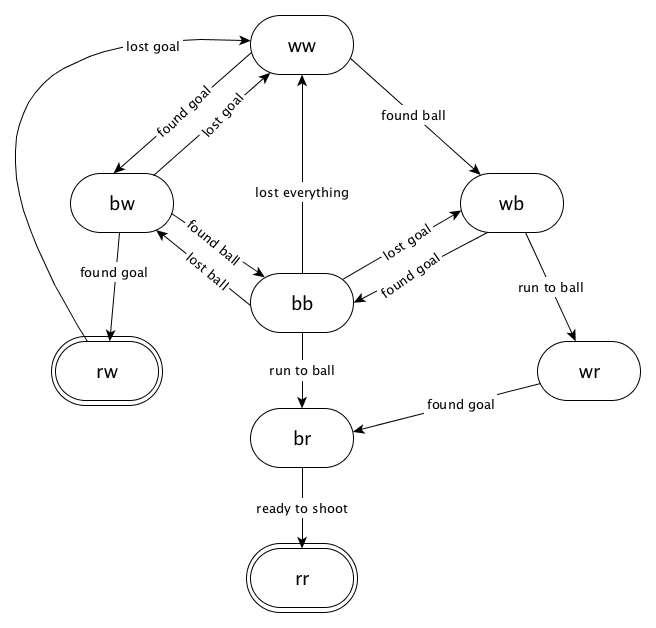
\includegraphics[scale=.5]{stateDiagram.png} 

\begin{tabular}{|p{.21\linewidth}|p{.3\linewidth}|p{.38\linewidth}|}
\hline
\cellcolor[gray]{0.5}\textcolor{white}{Shortcut} & \cellcolor[gray]{0.45}\textcolor{white}{Meaning} & \cellcolor[gray]{0.5}\textcolor{white}{Status}\\ \hline
ww&Left and right eye are white&The Nao can't see the ball or the goal\\ \hline
bw&Left eye blue, right eye white&The Nao has found the goal but no ball \\ \hline
bb&Left and right eye are blue&Has found goal and ball, but to far away for kick \\ \hline
wb&Left eye white, right eye blue&The Nao has found the ball but not the goal\\ \hline 
rw&Left eye red, right eye white&Nao tells other teammates where the goal is \\ \hline
br&Left eye blue, right eye red&The Nao has the ball and found the goal and it is on the way to the ball\\ \hline
wr&Left eye white, right eye red&The Nao plans to access the ball, this is only possible if the left eye was blue before\\ \hline
rr&Left and right eye are red&The Nao kick the ball to the goal, only after the blue-red status\\ \hline
\end{tabular}

\subsubsection{Recognition of Obstacles}
We have seen so far that an essential part during a game is to detect other players, the goal post, etc. Because if a robot runs into an object it mostly falls down. The currently playing teams do their image analysis based on typical edge detection strategies like convolution matrices, Canny edge detection, etc. So, it seems to be worth investigating whether the use of spectral analytical models like Fourrier transforms or Wavelets could gain any competitive advantage.

\subsubsection{Player to Player Communication}
In order to have a basis for a useful work split between the four different team players on the field (not the goalie) it is necessary to get the status between the robots exchanged. This will be done via the local Wifi which is permitted by the rule set. We consider it useful to exchange player and ball coordinates and the different status of the individual Naos.

\subsubsection{Integration of GameController}
The GameController is the head of the game and sends different signals, like game status, penalty states, etc. to the Naos. The Naos have to react on these. This part of the software is considered to be one of the less critical ones.

\subsubsection{Self Location and Orientation on the Field}
Another central topic to get an effective Nao team done is to provide each Nao with the clear and distinct information about his position on the field and where the own and the opponent's half is. In order to do so want to set-up a virtual coordinate system of the playing field, which is shared by all Naos during the game. The initial setup of this coordinate system is done during the “Ready”-phase since at this point all Naos know where their half of the field is and, therefore, can determine a common and distinct point of origin. Based on this every Nao broadcasts its position and the position of the ball (if the Nao sees the ball). As long as the data is in sync and no contradictions appear we might be pretty sure that all Naos are on track. If contradictions occur or a Nao comes back from “Penalized”-state a majority-wins-strategy will be applied to re-sync all Naos to a consistent coordinate system.

%At the start of the game (called 'Set') the robots have to go to their field position. The robots would be able to use a short time to scan the field from the Set phase via their camera. This means for instance that the robots know on which half they play, where the goal is located, etc. The field is for the robots like a coordinate system. During the game they are calculating where they are, where the ball is, etc. and send the coordinates to each other. So the robots are able to notice when they go into the wrong direction or anything like that. 

\subsubsection{Long Time Tests}
When monitoring the competition 2016 it became obvious that the top teams were able to keep their Naos stable until the end of each half time. This is not trivial since the joint temperatures raise heavily during one match. So we will have to focus on energy efficient movements to keep the joints as cool as possible, on the one hand and to save battery power, on the other hand. We expect to get most benefit by analyzing and adapting the most efficient walks from the teams of Australia and Austin, TX.

\subsubsection{Goal Keeper}
We observed that many teams have their goal keepers only standing between the posts and leaving it pretty inactive. However the top teams have a more active goalie which tries actively to catch the ball or, if possible, to throw the ball out of the penalty box by using its hand. We expect to be able to handle dangerous situations in our penalty box better if we adapt this kind of behavior.

\subsubsection{Recognition of the Referee's Whistle}
At the start of the game the referee blows a whistle and 15 seconds after this the game controller sends a start signal via wifi. If the Naos recognize the acoustic signal they have a competitive advantage. Here we expect to have some work in audio signal analysis, where a combination of frequency analysis (to distinguish the sound of the whistle from other rather loud sounds) and amplitude analysis (to distinguish from other high frequent sounds near the field) could be of help.

\subsubsection{Penalty Shootout}
The game is separated in two halves each taking 10 minutes. After these if the scores are the same the penalty shootout starts. How the penalty shootout works is described in the rule book~\cite{robocup_technical_committee_robocup_2016}. For this process an own software has to be written for one player and for the goal keeper. 


\section{Opportunities and Risks}
The following opportunities for our school can be listed.
\begin{itemize}
\item Publicity for the school to be attractive for talented new students
\item Publicity for the school to be attractive for the economic partners
\item Attractive field of study for students of the third, fourth and fifth grade
\end{itemize}
The following risks have to be taken into account.
\begin{itemize}
\item Late release of rule set compared to due date of application
\item Challenging topic which could get overwhelming
\item Relatively high financial input necessary
\end{itemize}

\section{Planning}
\subsection{Rough Schedule}

\begin{tabular}{|p{.2\textwidth}|p{.4\textwidth}|p{.32\textwidth}|}
\hline
\cellcolor[gray]{0.5}\textcolor{white}{Date} & \cellcolor[gray]{0.45}\textcolor{white}{Milestone} & \cellcolor[gray]{0.5}\textcolor{white}{DoD} \\ \hline
August 20, 2016 & Tool chain is installed on all team member's computers & Every team member can build a sample application, flash it and start it on the Nao \\ \hline
August 31, 2016 & Update Nao to current version & Upload the new software version on the Nao and rewrite the old code \\ \hline
September 2, 2016 & Overview of the different code parts from other teams & Every team member made a summery of the different code releases from other teams(B-Humans, UTAustin, UNSW Australia) \\ \hline
October 12, 2016 & Rewrite the current dances to the new version & Current dances have to work on the new version, so till Welser Messe they have to be functional \\ \hline
December 1, 2016 & Call for Application & deadline for application for participation \\ \hline
January 26, 2016 & Tag der offenen Tuer & demonstrate our current state of the soccer project \\ \hline
July 22, 2016 & Start of the trainee camp at the RoboCup & Everything has to work due to the start of the RoboCup\\ \hline
\end{tabular}


\subsection{Budget}
The budget is split into the two phases as described in section~\ref{sec:managementsummary}. To recall: Phase 1 is planned from now to December 10, 2016. In case we are able to successfully apply for the SPL 2017 in Nagoya the second phase would start by December 20, 2016 and last until July 27, 2017.
\subsubsection{Phase 1}
\begin{tabular}{|p{.6\linewidth}|r|r|r|}
\hline
\cellcolor[gray]{0.5}\textcolor{white}{Text} & \cellcolor[gray]{0.45}\textcolor{white}{Count} & \cellcolor[gray]{0.5}\textcolor{white}{Single Price} & \cellcolor[gray]{0.45}\textcolor{white}{Total} \\ \hline
Replacement for Sue (GEODE Nao) and Luc (oldest Atom Nao) & 2 & \euro{} 6,500.00 & \euro{} 13,000.00\\ \hline
Extra Battery Packs for available Naos & 4 & \euro{} 220.00 & \euro{} 880.00 \\ \hline
Artificial turf (approx. 60 $m^2$) & 60 & \euro{} 5.00 & \euro{} 300.00 \\ \hline
Web domain & 1 & \euro{} 12.00 & \euro{} 12.00 \\ \hline
Sum &  &  & \euro{} 14,180.00 \\ \hline
\end{tabular}

\subsubsection{Phase 2}
\begin{tabular}{|p{.6\linewidth}|r|r|r|}
\hline
\cellcolor[gray]{0.5}\textcolor{white}{Text} & \cellcolor[gray]{0.45}\textcolor{white}{Count} & \cellcolor[gray]{0.5}\textcolor{white}{Single Price} & \cellcolor[gray]{0.45}\textcolor{white}{Total} \\ \hline
Replacement for Judy (second Atom Nao) & 2 & \euro{} 3,500.00 & \euro{} 3,500.00\\ \hline
Four more Naos (Competition Price) & 4 & \euro{} 3,500.00 & \euro{} 14,000.00 \\ \hline
Extra Battery Packs for new Naos & 4 & \euro{} 220.00 & \euro{} 880.00 \\ \hline
Jerseys for Robots & 6 & \euro{} 25.00 & \euro{} 150.00 \\ \hline
Jerseys for Team & 8 & \euro{} 25.00 & \euro{} 200.00 \\ \hline
Travel costs to Nagoya (8 persons) & 8 & \euro{} 2,000.00 & \euro{} 16,000.00 \\ \hline
Maintenance costs for Naos & 2 & \euro{} 500.00 & \euro{} 1,000.00 \\ \hline
Sum &  &  & \euro{} 35,730.00 \\ \hline
\end{tabular}

\bibliography{my_bibliography}{}
\bibliographystyle{plainurl} % save alternatives are abbrvurl	alphaurl	plainurl	unsrturl
\end{document}  